\section{Introduction}\label{sec:intro}

\begin{figure*}[t]
\centering
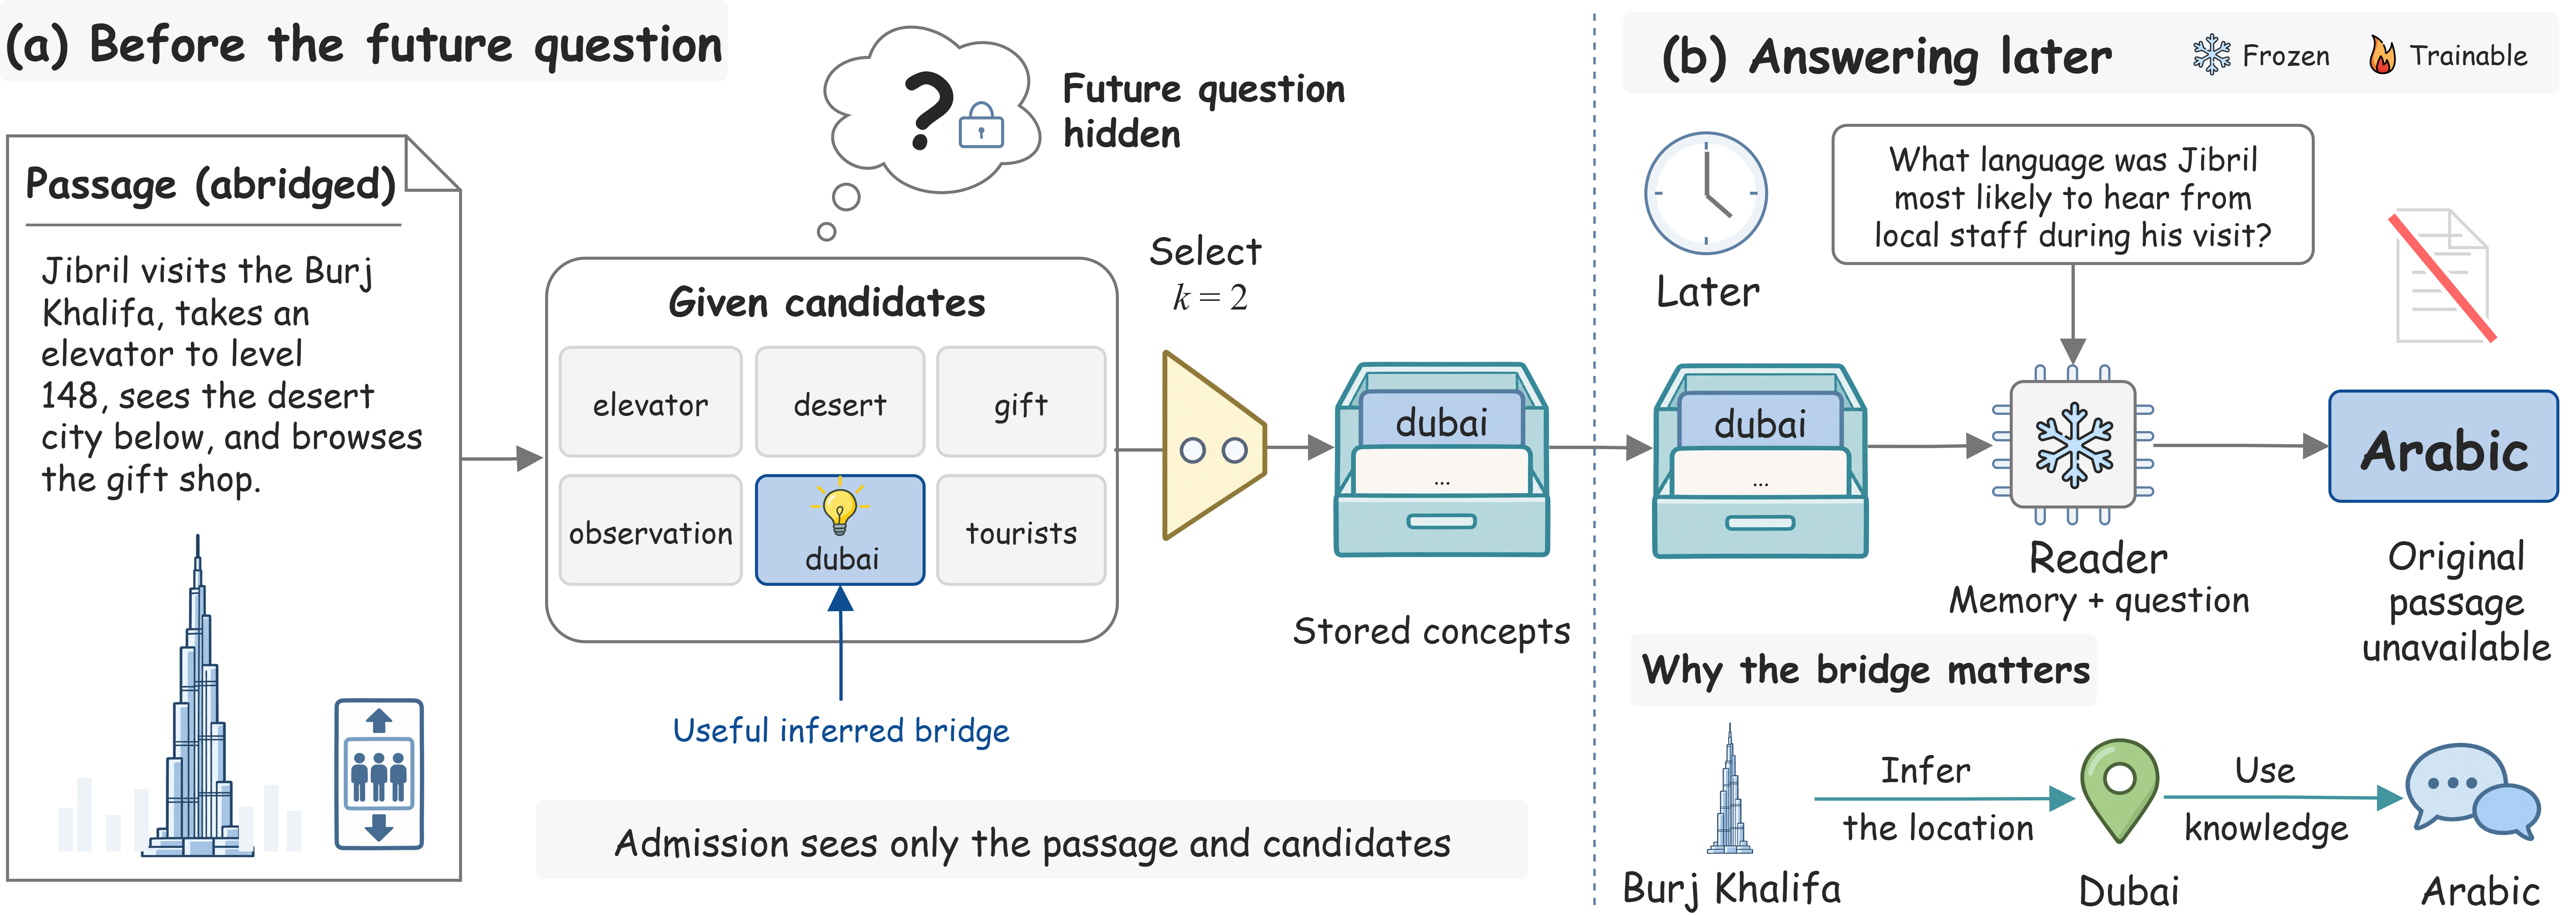
\includegraphics[width=\textwidth]{figures/fig3.png}
\caption{The Statedness Bias in one admission episode: the importance report keeps passage words. (a) Before the future question, each policy sees the passage and eight candidates, three stated and five unstated (the useful concept \texttt{mesopotamia} and four other ancient regions). Each stores two: importance report \{\texttt{silt}, \texttt{tablet}\}; unstated-first with report ordering \{\texttt{mesopotamia}, \texttt{levant}\}; SDA \{\texttt{mesopotamia}, \texttt{tablet}\}. (b) Later, the frozen reader sees only stored concepts and the question about the modern country Yara visited: importance report, no country determined; unstated-first with report ordering, Lebanon; SDA, Iraq; closed-book (no memory), United Kingdom. Qwen3-8B, statedness-balanced pool.}
\label{fig:episode}
\end{figure*}

External memory systems such as MemGPT, Mem0, and A-MEM let LLM agents retain information across interactions \citep{packer2023memgpt,mem0,amem2025}. Agents choose what to store under a budget before future questions arrive. Systems ask how important each candidate is through judgments such as Generative Agents' 1--10 importance rating \citep{park2023generative} and admission criteria such as ConsistencyGate and A-MAC \citep{consistencygate2026,amac2026}. Does the judgment track what a passage means, or only what it states? A future question that combines a passage with world knowledge depends on what the passage implies.

Figure~\ref{fig:episode} shows the consequence. Yara examines cuneiform tablets beside a river that fed early agriculture, but the passage never names Mesopotamia. A later question asks which modern country she visited. The yes/no importance report stores \texttt{silt} and \texttt{tablet}; the frozen reader cannot name a country. Storing \texttt{mesopotamia} and \texttt{tablet} instead lets it answer Iraq. Recovering \texttt{mesopotamia} requires a bridging inference \citep{haviland1974whatsnew}, linking the passage to prior knowledge. Naming that concept changes its statedness without changing its usefulness. Unstated-first with report ordering stores \texttt{mesopotamia} and \texttt{levant}, and the reader answers Lebanon: the other stored concept changes the reader's answer.

Readers remember the situation a text describes, including inferences, more than its wording \citep{bransford1972sentence,kintsch1988construction}. Memory admission must likewise separate statedness, whether a passage states a candidate, from usefulness, whether a future question needs it. Here, \texttt{silt} is stated but useless; \texttt{mesopotamia} is useful but unstated, or implied. Treating literal presence as evidence of importance changes what the agent can later answer. A diagnostic must distinguish failure to recognize a useful inference from failure to select it under a memory budget.

We hypothesize a \textbf{Statedness Bias}: importance judgments favor concepts because the passage states them. The importance prompt asks for passage support, which passage words provide directly; published admission criteria score that support explicitly \citep{consistencygate2026,amac2026}. Conversational benchmarks such as LoCoMo and LongMemEval measure end-to-end memory performance without separating stated from implied information \citep{maharana2024locomo,wu2025longmemeval}. They evaluate whether a system retrieves and uses conversation content, leaving admission of implied concepts untested. Separating admission from the reader's later answer lets us attribute differences to what each policy stores.

Our diagnostic crosses useful-concept and distractor statedness (\S\ref{sec:design}). Win rate measures within-episode comparisons in which the useful concept outranks a distractor, counting ties half. Comparing an implied useful concept against stated distractors exposes the bias; comparing it against unstated distractors tests recognition. We evaluate ranking and frozen-reader accuracy on a statedness-balanced pool, where statedness alone ranks at chance, and the original pool, where the useful concept is usually the only unstated candidate. All policies share candidate strings and a reader, so their answer differences arise from admission; the future question and answer remain hidden while candidates are scored. The diagnostic requires labeled episodes and a frozen reader and applies to any importance judgment. We evaluate six models from three families (7B to 32B) on 363 test episodes.

The Mesopotamia example is representative. The report ranks implied useful concepts above stated distractors in 38.3\% of comparisons versus 92.4\% against unstated distractors (Table~\ref{tab:grid}). The rating also shows the Statedness Bias; ConsistencyGate and A-MAC utility favor stated candidates. Statedness-cued wording reverses the preference. The model recognizes implied useful concepts, while its logit-lens readout and output likelihood show weaker statedness preference. Self-Distilled Admission (SDA) trains the importance judgment on these signals through an admission-only LoRA adapter \citep{hu2021lora}, raising implied useful-concept retention from 33.4\% to 63.8\% with two stored concepts while also improving stated retention (Table~\ref{tab:splitfull}).

SDA exceeds the report in 18 original-pool model-budget comparisons and gains 11.0 accuracy points on Qwen3-8B's enlarged pool at the two-concept budget (App.~\ref{app:poolresults}).

Our contributions are as follows:
\begin{itemize}
\item We identify the Statedness Bias: importance judgments favor passage words despite recognizing implied useful concepts.
\item We introduce a statedness diagnostic and SDA, which trains admission on the model's own signals.
\item SDA removes the strong form and exceeds the report and rating in all 18 model-budget comparisons on the statedness-balanced pool.
\end{itemize}
